% !TeX root = RJwrapper.tex
\title{\CRANpkg{lg}: An R package for Local Gaussian Approximations}
\author{by H{\aa}kon Otneim}

\maketitle

\abstract{
The package \CRANpkg{lg} for the R programming language provides implementations of recent methodological advances on applications of the local Gaussian correlation. This includes estimation of the local Gaussian correlation itself, multivariate density estimation, conditional density estimation, various tests for independence and conditional independence, as well as a graphical module for creating dependence maps. This paper describes the \CRANpkg{lg} package, its principles and its practical use.
}

\section{Introduction}

\citet{tjos:huft:2013} propose the \emph{local Gaussian correlation} (LGC) as a new measure of statistical dependence between two stochastic variables $X_1$ and $X_2$, which has the following important property yet unrivaled in the literature: It can separate between positive and negative nonlinear dependence while still reducing to the ordinary Pearson's correlation coefficient if $X_1$ and $X_2$ are jointly normally distributed. The R-package \CRANpkg{localgauss} \citep{bere:klep:tjos:2014} provides two important functions in this context; one that calculates the sample LGC based on observed values of $(X_1,X_2)$, and one that uses the estimated LGC to perform a local test of independence between $X_1$ and $X_2$ as described in detail by \citet{bere:tjos:2014}.  

We have lately seen a number of new applications of the LGC that the \CRANpkg{localgauss}-package does not support, however. \citet{stov:tjos:huft:2014} use the LGC to test for financial contagion across markets during crises. \citet{otne:tjos:2017} present a procedure for estimating multivariate density functions via the LGC, which \citet{otne:tjos:2018} modify in order to compute estimates of conditional density functions. \citet{laca:tjos:2017} present a test for serial independence within a time series, which \citet{laca:tjos:2018} extend in order to include a test for cross-correlation between two time series. Finally, \citet{otne:tjos:2019} develop the local Gaussian \emph{partial} correlation (LGPC) as a measure of conditional dependence, and a corresponding test for conditional independence. 

This paper describes the \CRANpkg{lg}-package \citep{otne:2019}, which provides a unified framework to implement all these methods, as well as a tool for visualizing the LGC and LGPC as dependence maps (and conditional dependence maps). \citet{jord:tjos:2017} use the LGC in spectral analysis of time series, but those methods have their own computational ecosystem in the \pkg{localgaussSpec}-package, \citet{jord:2018}.

In Section \ref{chap:background} we provide a brief introduction to the LGC as well as the methods and applications referred to above. In Section \ref{chap:lgobject} we describe the core function in the \CRANpkg{lg}-package and move on to demonstrate the implementation of various applications in Section \ref{chap:inference}. We conclude this paper in Section \ref{chap:graphics} by demonstrating the graphical capabilities of the \CRANpkg{lg}-package.

\section{Statistical background} 
\label{chap:background}

Consider a random vector $X$ having the unknown probability density function $f_X(x)$. It is a standard task to estimate $f_X$ based on a random sample $X_1,\ldots, X_n$, and the statistical literature provides an abundance of methods to accomplish this. One may, for example, make the assumption that the unknown density function has a particular parametric form, $f_X \in F_{\theta}$, where $F_{\theta} = \{f(x;\theta), \theta \in \Theta\}$ is a family of probability density functions indexed by some parameter $\theta$, and where $\Theta$ is the parameter space. Under this assumption we will typically produce an estimate of the parameter $\theta$, written $\widehat \theta$, using the maximum likelihood method. The estimated probability density function is then given as $\widehat f_X(x) = f(x; \widehat\theta)$.

A different approach is to estimate $f_X(\cdot)$ without any prior parametric assumptions. The classical method for non-parametric denstity estimation is the kernel estimator 
$$\widehat f_X(x) = \frac{1}{nb}\sum_{i=1}^n K\left(\frac{X_i - x}{b}\right),$$
where $K$ is a symmetric density function (the kernel) and $b$ is a tuning parameter (the bandwidth) that controls the smoothness of the estimate $\widehat f_X(\cdot)$. See \citet{silv:1986} for an introduction to this topic. There is also a massive statistical literature on density estimation containing extensions and improvements to the classical methods to be used in various practical situations. 

\citet{hjor:jone:1996} provide one such idea. They consider a parametric family $F_{\theta}$, but instead of searching for a single parameter value $\theta_0$, for which $f_X(x) = f(x;\theta_0)$ (or approximately so), they rather assert that different members of $F_{\theta}$ may approximate $f_X$ locally in different parts of its domain. In other words, they seek to estimate a parameter \emph{function} $\theta_0(x)$ for which $f_X(x) = f(x;\theta_0(x))$ (or approximately so), and do this by maximizing a \emph{local likelihood function} in each point $x$:
\begin{align}
\widehat\theta(x) 
&= \arg\max_{\theta \in \Theta} L_n(\theta, x) \nonumber\\ 
&= \arg\max_{\theta \in \Theta} \frac{1}{nb}\sum_{i=1}^n K\left(\frac{X_i - x}{b}\right)\log f(X_i; \theta) - \int \frac{1}{b}K\left(\frac{y - x}{b}\right)f(y;\theta)\,\textrm{d}y,
\label{eq:loclik}
\end{align}
where, again, $K$ is a symmetric density function and $b$ is a bandwidth parameter that controls the smoothness of the estimate. The second term in the local likelihood function is a penalty that ensures that the estimated density $\widehat f_X(x) = f(x; \widehat\theta(x))$ converges correctly to the true density function $f_X(x)$ as the sample size $n$ increases to infinity and the bandwidth $b$ decreases towards zero. See \citet{hjor:jone:1996} for a detailed discussion about this construction.

\citet{tjos:huft:2013} consider the bivariate case $X = (X_1, X_2)$ and take $F_{\theta}$ to be the family of bivariate normal distributions consisting of densities on the form

\begin{align}
f(x;\theta) 
&= \psi(x_1, x_2;\mu_1, \mu_2, \sigma_1, \sigma_2, \rho)  \nonumber\\ 
&= \frac{1}{2\pi \sigma_1 \sigma_2\sqrt{1-\rho^2}} \nonumber \\
& \qquad \times\exp \left\{-\frac{1}{2(1-\rho^2)}\left(\frac{(x_1-\mu_1)^2}{\sigma_1^2}-2\rho\frac{(x_1-\mu_1)(x_2-\mu_2)}{\sigma_1 \sigma_2}+\frac{(x_2-\mu_2)^2}{\sigma_2^2}\right)\right\},
\label{eq:gaussian}
\end{align}
where $\theta = (\mu_1,\mu_2,\sigma_1,\sigma_2,\rho)$ is the vector of parameters. Using a sample $\{X_{1i}, X_{2i}\}$, $i = 1, \ldots, n$, they estimate $\theta$ locally in the point $x$ by maximizing the local likelihood function \eqref{eq:loclik}, producing
$$\widehat\theta(x) = (\widehat\mu_1(x), \widehat\mu_2(x), \widehat\sigma_1(x), \widehat\sigma_2(x), \widehat\rho(x)),$$
and take special interest in the estimated correlation function $\widehat\rho(x)$ (i.e. the LGC) because it serves as an attractive local measure of statistical dependence between $X_1$ and $X_2$. They show that the LGC reveals many types of nonlinear statistical dependence that are not captured by the ordinary (global) Pearson correlation coefficient. Furthermore, the LGC distinguishes between positive and negative dependence and reduces to the Pearson $\rho$ if $X_1$ and $X_2$ are jointly normal. We refer to \cite{tjos:huft:2013} for a detailed treatment of the theoretical foundations of the LGC as well as several examples, and rather present two simple illustrations at this point in order to demonstrate the concept. 

\begin{figure}[t]
    \centering
    \begin{subfigure}[t]{0.48\textwidth}
      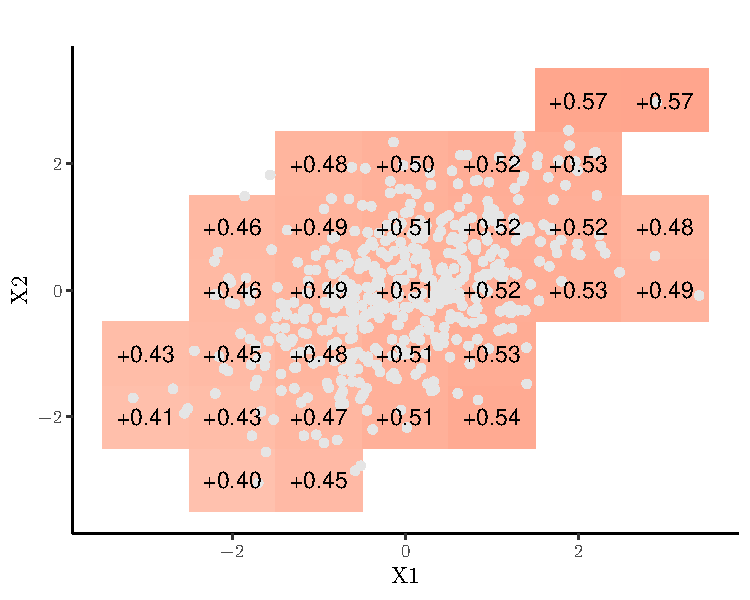
\includegraphics[width=\textwidth]{gaussian-example}
      \caption{Estimated local Gaussian correlations between two  jointly normal variables having correlation equal to 0.5, based on 1000 observations.}
    \end{subfigure}
    \begin{subfigure}[t]{0.48\textwidth}
      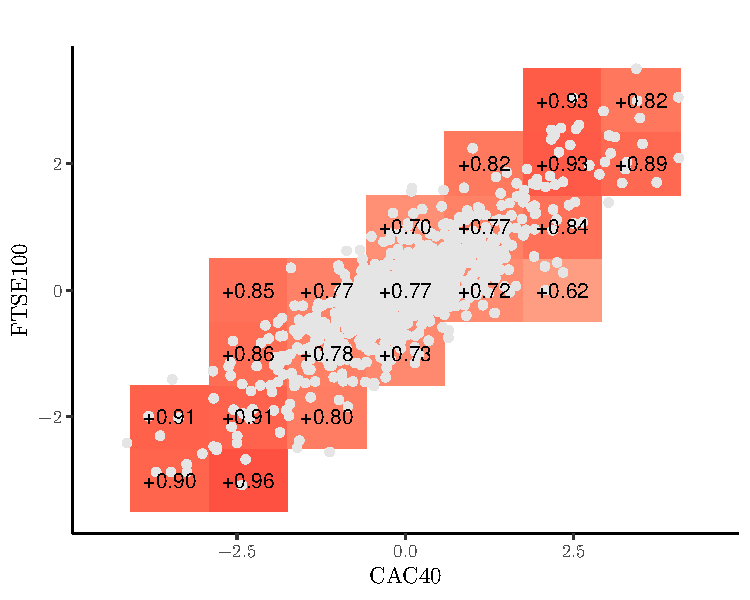
\includegraphics[width=\textwidth]{returns-example}
      \caption{Local Gaussian correlation between daily returns from the CAC40 and FTSE100 stock indices, based on 1000 consecutive trading days.}
    \end{subfigure}
    \caption{Two dependence maps}
    \label{fig:initial-example}
  \end{figure}
  
In Figure \ref{fig:initial-example} we have plotted the estimated LGC for two bivariate data sets on a grid; 1000 simulated observations from a binormal distribution having correlation equal to 0.5, and the daily return on the CAC40 and FTSE100 stock indices on 1000 consecutive trading days starting on May 5th 2014. In the first panel, we see that the estimated local correlation coincides with the global correlation, except for the estimation error. In the second panel we see clearly that the local correlation, and thus the dependence, is stronger in the lower left and upper right regions of the distribution than in central parts. The phenomenon of local dependence is well known in the financial literature, and using the LGC it can be measured, interpreted, and visualized in a natural way. The interpretation of this particular figure is that extreme observations on the two stock indices are more strongly dependent than the less extreme observations. 

One may obtain these particular estimates from the older \CRANpkg{localgauss}-package (as well as the \CRANpkg{lg}-package of course), but the plotting routine that was used to produce these figures is included in the \CRANpkg{lg}-package and will be described in more detail in Section \ref{chap:graphics}.

Taking the LGC as a measure of dependence opens up for a number of possibilities to construct statistical tests. \citet{bere:tjos:2014} show that $\rho(x) \equiv 0$ implies that $X_1$ and $X_2$ are independent. The converse statement holds if $\mu_i(x_1, x_2) = \mu_i(x_i)$ and $\sigma_i(x_1, x_2) = \sigma_i(x_i)$ for $i=1,2$, and in general if the observations have been suitably transformed according to a procedure presented later in this section. It follows then that departures from $\widehat\rho(x) \equiv 0$ may be taken as evidence against the hypothesis that $X_1$ and $X_2$ are statistically independent. \citet{bere:tjos:2014} formalize this notion by testing whether $\rho(x) \equiv 0$ for all $x\in S \subset \mathbb{R}^2$ using the test statistic

\begin{equation}
T_{n,b} = \int_S h\left(\widehat \rho(x) \right) \,\textrm{d}F_n(x)
\label{eq:test-statistic1}
\end{equation}
for some non-negative function $h$, for example $h(x) = x^2$ or $h(x) = |x|$. Critical values may be obtained by permutations of the data under the null hypothesis, and we demonstrate the implementation of this test using the \CRANpkg{lg}-package in Section \ref{chap:indtests}.

Consider next the stationary time series $\{X_t\}$. The autocorrelation function (ACF) $\rho_k = \rho(X_t, X_{t-k})$ is a well known concept for describing the serial dependence in the time seris, but the ACF is, again, only capable to completely capture \emph{linear} serial dependence. \citet{laca:tjos:2017} seek to remedy this by rather calculating the the local correlation between $X_t$ and $X_{t-k}$. This leads to a test for serial independence in the natural way. In fact, this work is mainly a theoretical exercise in order to accommodate time series dependence. Testing for independence between $X_t$ and $X_{t-k}$ using observations $\{X_t, X_{t-k}\}_{t = k+1}^T$ leads to the same test statistic \eqref{eq:test-statistic1} and bootstrap procedure as the test for independence between $X_1$ and $X_2$ that we described above. 

\citet{laca:tjos:2018} extend this problem to test for serial cross-dependence between two time series $\{X_t, Y_t\}$ by measuring the LGC between $X_t$ and $Y_{t-k}$. Departures from $\widehat\rho(x,y) \equiv 0$ is again taken as evidence against independence, and the test statistic (\ref{eq:test-statistic1}) provides an aggregate measure of this discrepancy in the specified region $S$. In this case, however, we can not obtain replicates of the test statistic under the null hypothesis by simple permutations of the data. \citet{laca:tjos:2018} suggest rather two block bootstrap procedures to this end, using fixed and random block sizes respectively. The tests for serial dependence, and serial cross-dependence are both implemented in the \CRANpkg{lg}-package, as we demonstrate in Section \ref{chap:indtests}.

We find another application of the local Gaussian approximation in the work by \citet{stov:tjos:huft:2014}, who measure and test for financial contagion. They define contagion by "a significant increase in cross-market linkages after a shock to one country" \citep{forb:rigo:2002} and employ the LGC to quantify this potential linkage. The authors estimate the LGC on a grid $\{x_1, x_2\}_k$, $k=1,\ldots,K$ along the diagonal $D=\{(x_1,x_2): x_1 = x_2\}$ \emph{before} and \emph{after} some critical event in the financial markets, denoted as the crisis (C) and the non-crisis (NC) periods respectively. They compare the two estimates using the following test statistic; 

$$T_{n,b}^D = \sum_{k=1}^K \left\{\widehat\rho_C(x_k, x_k) - \widehat\rho_{NC}(x_k, x_k) \right\}w(x_k,x_k),$$

where $w(\cdot, \cdot)$ is a weight function that serve the same purpose as the integration area $S$ in (\ref{eq:test-statistic1}). In this case, \citet{stov:tjos:huft:2014} show that a standard bootstrap will suffice in order to produce approximate replicates of $T_{n,b}^D$ under the null hypothesis of no financial contagion, and we demonstrate the implementation of this test using the \CRANpkg{lg}-package in Section \ref{chap:cont}.

Although the original work by \citet{hjor:jone:1996} provide a general framework for local likelihood density estimation, using any $p$-variate parametric family as the local family, it is evident that the method may struggle in multivariate applications much in the same way as the kernel density estimator does. This is a consequence of the curse of dimensionality, the effect of which is sought remedied by an algorithm provided by \citet{otne:tjos:2017}. The idea is to fit the $p$-variate normal distribution $\psi(\mu, \Sigma)$ locally, where $\mu$ is the vector of $p$ expectations, and $\Sigma$ is the $p\times p$ covariance matrix (to which the correlation matrix $R$ corresponds), but under the following structural simplifications:

\begin{align}
\mu_i(x) &= \mu_i(x_1, \ldots, x_p) \stackrel{\textrm{def}}{=} \mu_(x_i) \label{eq:simp-mu}\\
\sigma_i(x) &= \sigma_i(x_1, \ldots, x_p)  \stackrel{\textrm{def}}{=} \sigma_i(x_i) \label{eq:simp-sig} \\
\rho_{ij}(x) &= \rho_{ij}(x_1, \ldots, x_p) \stackrel{\textrm{def}}{=} \rho_{ij}(x_i, x_j). \label{eq:simp-rho}
\end{align}
\citet{otne:tjos:2017} estimate the local parameters above by first obtaining univariate marginal locally Gaussian fits (eqs. \ref{eq:simp-mu} and \ref{eq:simp-sig}), and then pairwise bivariate locally Gaussian fits (eq. \ref{eq:simp-rho}). In the second step the estimates $\widehat\mu_i(x_i)$, $\widehat\mu_j(x_j)$, $\widehat\sigma_i(x_i)$ and $\widehat\sigma_j(x_j)$ are kept fixed in the estimation of the pairwise local correlation. They argue further that the following transformation technique will produce better density estimates in many situations. Denote by $F_i(x_i)$, $i = 1,\ldots, p$ the marginal distribution functions of the stochastic vector $X$, and by $\widehat F_i(x_i) = n^{-1}\sum_{i=1}^n 1(X_i \leq x_i)$ their empirical counterparts. They then estimate the density $f_Z(z)$ of the vector $Z = \{\Phi^{-1}(F_i(X_i))\}_{i=1,\ldots,p}$, in practice approximated by 

\begin{equation}
\widehat Z = \{\Phi^{-1}(\widehat F_i(X_i))\}_{i=1,\ldots,p}, 
\label{eq:trans}
\end{equation}
and where $\Psi(\cdot)$ is the univariate standard normal cdf. In that case, they simplify the estimation problem even further and fix

\begin{equation}
\mu_i(z_i) \stackrel{\textrm{def}}{=} 0 \,\, \textrm{ and } \sigma_i(z_i) \stackrel{\textrm{def}}{=} 1, \,\, i = 1,\ldots,p,
\label{eq:simp}
\end{equation}
so that the only parameter functions left to estimate are the pairwise local Gaussian correlations $R(z) = \{\rho_{ij}(z_i, z_j)\}_{i<j}$. We use the notation $Z$, $z_i$ and $z_j$ to signify that the estimation is performed on the (approximate) standard normal scale, or $z$-scale for short. We can then estimate the joint density $f_Z(z)$ of $Z$ as
\begin{equation}
\widehat f_Z(z) = \psi(z; \mu = 0, \sigma = 1, R = \widehat R(z)),
\label{eq:transformed-density}
\end{equation}
and then substitute $f_Z$ for $\widehat f_Z$ in the following relation obtained by \citet{otne:tjos:2017} in order to estimate the unknown density $f_X$:
\begin{equation}
f(x) = f_{Z}\big(\Phi^{-1}(F_1(x_1)), \ldots, \Phi^{-1}(F_p(x_p))\big) \times \prod_{i=1}^p \frac{f_i(x_i)}{\phi\big(\Phi^{-1}(F_i(x_i))\big)},
\label{eq:backtrans}
\end{equation}
where $\phi(\cdot)$ is the standard normal pdf. This estimator is implemented the \CRANpkg{lg}-package as demonstrated in Section \ref{chap:density}.

One particular feature enjoyed by the jointly normally distributed vector $X$ is that, for any partitioning $X = \left(X^{(1)}, X^{(2)}\right)$, the conditional distribution of $X^{(1)}|X^{(2)} = x^{(2)}$ is also normal. In fact, if $X \sim \mathcal{N}(\mu,\Sigma)$, and $\mu$ and $\Sigma$ is partitioned according to $\left(X^{(1)}, X^{(2)}\right)$ as
$$\mu = \begin{pmatrix} \mu_1 \\\mu_2 \end{pmatrix} \,\, \textrm{ and } \,\, \Sigma = \begin{pmatrix} \Sigma_{11} & \Sigma_{12} \\ \Sigma_{21} & \Sigma_{22} \end{pmatrix},$$
then $X^{(1)}|X^{(2)} = x^{(2)} \sim \mathcal{N}(\mu^*, \Sigma^*)$, where

\begin{align}
\mu^* &= \mu_1 + \Sigma_{12}\Sigma_{22}^{-1}\left(x^{(2)} - \mu_2\right) \label{eq:cond-mu} \\
\Sigma^* &= \Sigma_{11} - \Sigma_{12}\Sigma_{22}^{-1}\Sigma_{21}, \label{eq:cond-sig}
\end{align}
see e.g. \citet[chapter 4]{john:wich:2007}. \citet{otne:tjos:2018} demonstrate that this property may be translated into a corresponding local argument without modification. That is, if the joint density $f_X(\cdot)$ can be written on a locally Gaussian form 

$$f_X(x) = \psi(x, \mu(x), \Sigma(x)),$$

then the conditional density of $X^{(1)}|X^{(2)} = x^{(2)}$ can also be written on the same locally Gaussian form with local parameters given by equations (\ref{eq:cond-mu}) and (\ref{eq:cond-sig}), except that all quantities are $x$-dependent. If we use the transformation technique described above together with simplification (\ref{eq:simp}), the local versions of equations (\ref{eq:cond-mu}) and (\ref{eq:cond-sig}) simplify to

\begin{align}
\mu^*(z) &= R_{12}(z)R_{22}(z)^{-1}z^{(2)},  \label{eq:cond-mu-trans}\\
\Sigma^*(z) &= R_{11}(z) - R_{12}(z)R_{22}(z)^{-1}R_{21}(z), \label{eq:cond-sig-trans}
\end{align}
where we, again, switch to $z$-notation in order to make it clear that these quantities are estimated on the standard normal $z$-scale. An estimator $\widehat f_{X^{(1)}|X^{(2)}}(\cdot|\cdot)$ of the conditional density $f_{X^{(1)}|X^{(2)}}(\cdot|\cdot)$ follows immediately from an expression corresponding to (\ref{eq:backtrans}), and the \CRANpkg{lg}-package provides functions for implementing this estimator in R, and we describe the implementation of this functionality in Section \ref{chap:density}.

Finally, we refer to \citet{otne:tjos:2019}, who take the local version of the conditional covariance matrix (\ref{eq:cond-sig}) (or (\ref{eq:cond-sig-trans}) in the transformed case) as a measure for conditional dependence, and thus as an instrument to test for conditional independence. Consider the stochastic vector $X = \left(X^{(1)}, X^{(2)}, X^{(3)}\right)$, where $X^{(1)}$ and $X^{(2)}$ are scalars and $X^{(3)}$ may be a vector. $X^{(1)}$ is conditionally independent from $X^{(2)}$ given $X^{(3)}$, written $X^{(1)} \perp X^{(2)} \,|\,X^{(3)}$, if the stochastic variables $X^{(1)}\,|\,X^{(3)}$ and $X^{(2)}\,|\,X^{(3)}$ are independent, or, equivalently, if the joint conditional density of $X^{(1)}$ and $X^{(2)}$ given $X^{(3)}$ can be written as the product

\begin{equation}
f_{X^{(1)},X^{(2)}|X^{(3)}}\left(x^{(1)}, x^{(2)}|x^{(3)}\right) = f_{X^{(1)}|X^{(3)}}\left(x^{(1)}|x^{(3)}\right) \times f_{X^{(2)}|X^{(3)}}\left(x^{(2)}|x^{(3)}\right).
\label{eq:cond-ind}
\end{equation}
In this case, denote by $\alpha(z)$ the off-diagonal element in the $2\times2$ local correlation matrix $R^*(z)$ (which derives directly from $\Sigma^*(z)$ as given in (\ref{eq:cond-sig-trans})). If $X$ has a local Gaussian distribution, the conditional independence (\ref{eq:cond-ind}) is equivalent to $\alpha(z) \equiv 0$, and \citet{otne:tjos:2019} take departures from this relation as evidence against the hypothesis of conditional independence between $X^{(1)}$ and $X^{(2)}$ given $X^{(3)}$. The natural way to quantify this is the test functional

\begin{equation}
T^{CI}_{n, b} = \int h(\widehat\alpha(z)) \, \textrm{d}F_n(z).
\label{eq:ci-test-statistic}
\end{equation}
\citet{otne:tjos:2019} describe a bootstrap procedure for generating replicates of $T_{n,b}^{CI}$ under the null hypothesis. In Section \ref{chap:partial} we demonstrate how the \CRANpkg{lg}-package may be used to extract estimates of the local partial correlation and perform tests for conditional independence according to this scheme.

\section{The first step: Creating the \texttt{lg}-object} 
\label{chap:lgobject}

The local Gaussian correlation may be used to perform a number of statistical analyses, as is evident from the preceding section. The practitioner must first, however, make three quite specific modelling choices; namely (i) to choose an estimation method, i.e. the level of simplification in multivariate applications, (ii) to determine whether the data should be transformed towards marginal standard normality before estimating the LGC, and (iii) to choose a set of bandwidths, or at least a method for calculating bandwidths. The architecture of the \pkg{lg}-packages requires the user to make these choices \emph{before} endeavoring further into specific applications by imposing a strict, two step procedure:

\begin{itemize}
\item[1.] Create an lg-object.
\item[2.] Apply relevant analysis functions to the lg-object.
\end{itemize}

In the following we assume that one has a \emph{data set} \code{x} loaded into the R workspace, which must be an $n\times p$ matrix (one column per variable, one row per observation), possibly including \code{NA}`s which will be excluded, or a data frame having the same dimensions. The fundamental syntax for creating an lg-object is \code{lg\_object <- lg\_main(x)}, and we will in this section explain how the modelling decisions (i)-(iii) can be encoded into the lg-object.

\subsection{Selecting the estimation method}
\label{chap:est-method}

Given a data set \code{x} having $n$ rows and $p \geq 2$ columns, the user must choose between four distinct estimation methods, and specify this choice by using the argument \code{est\_method} to the \code{lg\_main()}-function. We look at the built-in bivariate data set `faithful` and load the \CRANpkg{lg}-package in order to demonstrate the implementation:

\begin{example}
R> x <- faithful
R> library(lg)
\end{example}

\textbf{1. A full locally Gaussian fit for bivariate data.} If $p = 2$, we may fit the bivariate normal $\psi(x, \theta)$ locally to $f(x)$, and by a "full local fit" we mean that we jointly estimate the five parameters
$$\theta(x) = \big(\mu_1(x_1, x_2), \mu_2(X_1, x_2), \sigma_1(x_1, x_2), \sigma_2(x_1,x_2),\rho(x_1, x_2)\big)$$
by optimizing the local likelihood function (\ref{eq:loclik}) in the grid point $x = (x_1, x_2)$. To use this estimation method in the subsequent analysis, specify \code{est\_method = "5par"} in the call to \code{lg\_main()}:

\begin{example}
R> lg_object <- lg_main(x, est_method = "5par")
\end{example}
The resulting \code{lg\_object} is a list of class \code{lg}, and we may confirm that the assignment has been carried out correctly by inspecting its \code{est\_method}-element:
\begin{example}
R> lg_object$est_method 

[1] "5par"
\end{example}

Note that the full locally Gaussian fit for raw data is not available if the number of variables $p$ is greater than 2. The \code{lg\_main()}-function will check for this and throw an error if $p>2$ and \code{est\_method = "5par"}.

\textbf{2. A simplified locally Gaussian fit for multivariate data.} As described in the preceding section, we may construct a simplified estimation procedure for calculating the LGC in two steps, which in principle works for any number of dimensions (including $p=2$):

\begin{itemize}
\item[1.] Calculate $\mu_i(x_i)$ and $\sigma_i(x_i)$, $i = 1,\ldots,p$ by fitting the univariate normal distribution locally to each \emph{marginal} density $f_i(x_i)$ of $f(x)$.
\item[2.] Keep $\widehat\mu_i(x)$ and $\widehat\sigma_i(x_i)$, $i=1,\ldots,p$ from step 1 fixed when estimating $\rho_{ij}(x_i, x_j)$, $1\leq i<j\leq p$ by fitting the bivariate normal distribution to each \emph{pair} of variables $X_i$ and $X_j$.
\end{itemize}
To use this method, create the lg-object by running the following line:

\begin{example}
R> lg_object2 <- lg_main(x, est_method = "5par_marginals_fixed")
\end{example}

\textbf{3. A simplified locally Gaussian fit for marginally standard normal data.} This estimation method is applicable for marginally standard normal data, or data that have been transformed to approximate marginal standard normality by e.g. the transformation (\ref{eq:trans}). In that case, we fix the marginal expectation functions and standard deviation functions to the constant values $0$ and $1$ respectively, rather then estimating them. To use this estimation method, create the lg-object by running

\begin{example}
R> lg_object3 <- lg_main(x, est_method = "1par")
\end{example}

Note that the function call above will issue a warning if the option for transforming the data to marginal standard normality is not at the same time set to \code{TRUE}, see the next sub-section for details.

\textbf{4. A full locally Gaussian fit for trivariate data.} If $p = 3$ \emph{and} we choose to transform the data to marginal standard normality (see the next sub-section), the transformed density $f_Z(\cdot)$ in (\ref{eq:transformed-density}) may be estimated by jointly estimating the three local correlations $\rho_{12}(z_1, z_2, z_3)$, $\rho_{13}(z_1, z_2, z_3)$ and $\rho_{23}(z_1, z_2, z_3)$. This estimation method was introduced recently by \citet{otne:tjos:2019} in order to increase power of their conditional independence test, but it can be used in any application described in this paper that consider trivariate data. To use this estimation method, create the lg-object by running

\begin{example}
R> lg_object4 <- lg_main(x, est_method = "trivariate")
\end{example}

\subsection{Data transformation}
\label{data-transformation}

\begin{figure}[t]
    \centering
    \begin{subfigure}[t]{0.48\textwidth}
      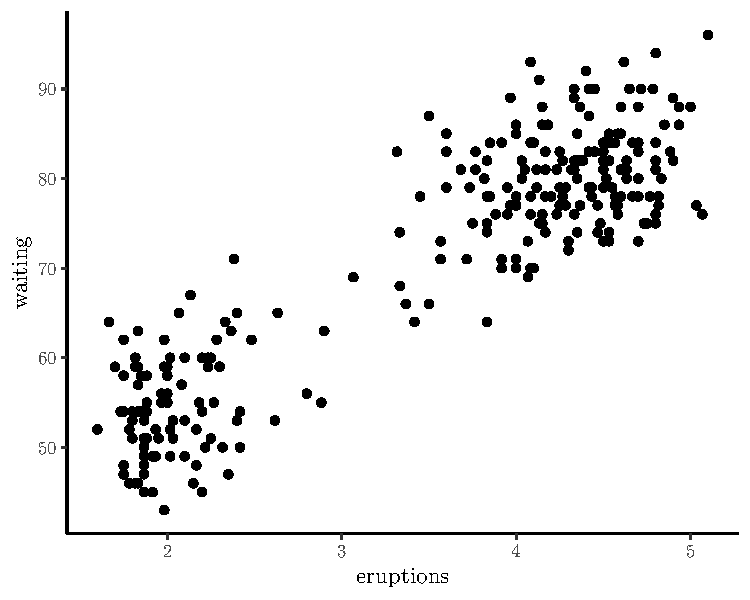
\includegraphics[width=\textwidth]{faithful}
      \caption{The original data.}
    \end{subfigure}
    \begin{subfigure}[t]{0.48\textwidth}
      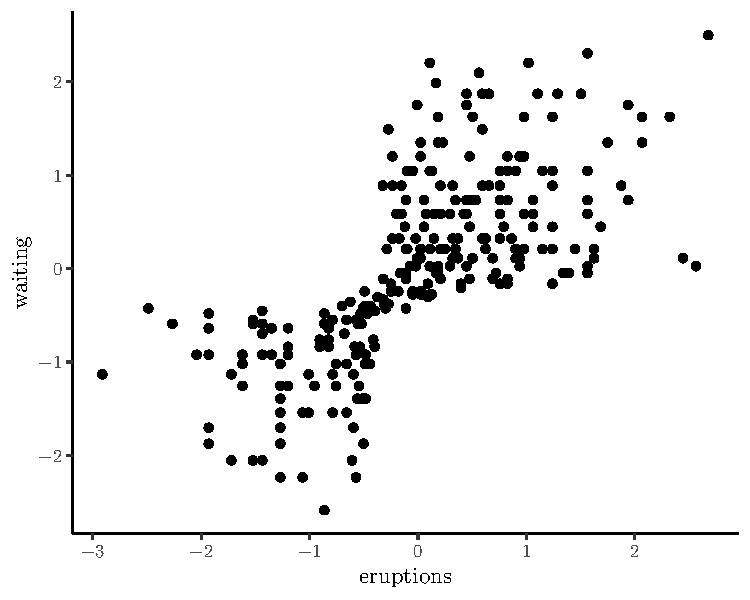
\includegraphics[width=\textwidth]{faithful-transformed}
      \caption{The same data transformed to marginal standard normality.}
    \end{subfigure}
    \caption{The same data on different scales.}
    \label{fig:faithful}
  \end{figure}


Next, the user must determine if the local Gaussian correlation should be estimated directly on the raw data or on the marginally normal pseudo observations \eqref{eq:trans}. This is carried out by using the logical \code{transform\_to\_marginal\_normality}-argument in \code{lg\_main}, for example:

\begin{example}
R> lg_object <- lg_main(x, transform_to_marginal_normality = TRUE)
\end{example}

The resulting \code{lg\_object} now includes the element \code{transform\_to\_marginal\_normality} set according to the input, and if this is \code{TRUE}, it also includes the \code{transformed\_data} and a function \code{trans\_new()} that may be used later to apply the same transformation to e.g. grid points. If the transformation option is set to \code{FALSE}, the \code{transformed\_data} element contains the input data \code{x}, and \code{trans\_new()} is nothing more than the identity mapping for points in \(\mathbb{R}^p\). See Figure \ref{fig:faithful} for two plots that demonstrate the effect of the data transformation on the example data.

\subsection{Bandwidth selection}\label{chap:bw}

Finally, the user must specify a set of bandwidths, or a method for calculating them. Given that the different estimation methods described in Section \ref{chap:est-method} require different sets of bandwidths (i.e joint, marginal and/or pairwise), the easiest approach for the user is to leave the selection and formatting of the bandwidths to the \code{lg\_main()}-function.

The bandwidth plays a slightly different role in local likelihood estimation than elsewhere in the nonparametric literature. It controls the \emph{level of localization} and thus only indirectly the \emph{smoothness} of the estimates. Indeed, if we concentrate on the univariate case for the moment and assume that the (single) bandwidth \(b\) is small, we see from the local likelihood function \eqref{eq:loclik} that only the very few observations closest to a fixed grid point \(x_0\) will have significant weight when determining the
local parameter estimates \(\widehat\theta_0(x)\) at that point. Moving on to another nearby point \(x_1\) may then lead to a fairly different estimate \(\widehat\theta(x_1)\) because the set of observations having weight in this point is very different. This may again lead to rougher parameter estimates \(\widehat\theta(x)\) and in turn also to rougher density estimates \(f(x,\widehat\theta(x))\).

If the bandwidth \(b\) grows large, on the other hand, all observations receive similar weights, and furthermore: the local likelihood function \eqref{eq:loclik} becomes approximately proportional to the ordinary (global) likelihood function \(L_n(\theta) = \sum_{i=1}^n\log f(X_i;\theta)\). In other words, the local parameter estimates \(\widehat \theta(x)\) are smoothed towards the constant maximum likelihood estimates \(\widehat\theta_{ML}\), and the estimated density \(f(x;\widehat\theta(x))\) towards the maximum likelihood estimate \(f(x;\widehat\theta_{ML})\). This means that the bandwidth may be chosen to reflect the goodness-of-fit of \(f(x;\theta)\) to the true density \(f(x)\).

In the multivariate applications referred to in this paper, the bandwidth \(b\) in \eqref{eq:loclik} is a diagonal matrix, and \(1/b\) is
naturally taken to represent its inverse. 

We have in practice seen two automatic bandwidth selectors employed in the applications referred to in Section \ref{chap:background}: a
cross-validation procedure, which is slow, but accurate with respect to density estimation, and a plug-in bandwidth that is quick, but cruder. We use the argument
\code{bw\_method} to the \code{lg\_main()}-function in order to choose between the two.

\textbf{1. Choosing bandwidths by cross-validation.} The functional

\[CV(b) = -\frac{1}{n}\sum_{i=1}^n \log f\Big(X_i; \widehat\theta^{(-i)}(X_i)\Big),\]
where \(\widehat\theta^{(-i)}(x)\) is the parameter estimate obtained after deleting observation \(X_i\) from the data, is proportional to a quantity that estimates the Kullback-Leibler distance between \(f(\cdot, \widehat\theta(\cdot))\) and the true density \(f(\cdot)\), see \citet{bere:tjos:2014}. The cross-validated bandwidth \(b_{CV}\) is hence given by \[b_{CV} = \arg\min_b \,\, CV(b).\] If we, for example, wish to use the simplified estimation procedure on the transformed data, we need bandwidths for the marginal estimates of the local means and standard deviations, as well as a \(2\times2\) diagonal bandwidth matrix for each pair of variables. This is accomplished by the following call to \code{lg\_main()}:

\begin{example}
R> # Create the lg-object with bandwidths chosen by cross-validation
R> lg_object <- lg_main(x,
R+                      est_method = "5par_marginals_fixed",
R+                      transform_to_marginal_normality = TRUE,
R+                      bw_method = "cv")
\end{example}

The \code{lg\_object} now contains the necessary bandwidths for this configuration, as can be seen by inspecting the contents of its
\code{bw}-element:

\begin{example}
R> # Print out the bandwidths
R> lg_object$bw

$marginal
[1] 0.9989327 0.9875333

$marginal_convergence
[1] 0 0

$joint
  x1 x2       bw1      bw2 convergence
1  1  2 0.2946889 0.331971           0
\end{example}
This is itself a list, containing the crucial elements \code{marginal} for the \(p\) marginal bandwidths, and \code{joint} that contains the
\(p(p-1)/2\) bandwidth matrices, one for each pair of variables (which in this bivariate example just \emph{one} variable pair, (\code{x1,\ x2})). The convergence flags stem from the \code{optim()} and \code{optimize()} functions that we use to obtain the minimizer of \(CV(\cdot)\), and 0 indicates successful convergence.

\textbf{2. Using plug-in bandwidths.} Obtaining cross-validated bandwidths is unfortunately fairly slow on a standard computer. For sample sizes in the 500-1000 range, the process may take several minutes, which is unfeasible when embarking on analyses that require e.g. resampling. We have therefore implemented a quick plug-in bandwidth selector as well, that may suffice in many practical situations, especially at the initial or exploratory stage. 

\citet{otne:tjos:2017} show that the simplified version of the local Gaussian fit have the same convergence rates as the corresponding nonparametric kernel density estimator, for which \citet{silv:1986} derives the plug-in formula \(b = 1.08\cdot sd(x) \cdot n^{-1/5}\). By
specifying \code{bw\_method\ =\ "plugin"}, the \code{lg\_main()}-function will select the bandwidths correspondingly, except that the exponent changes to \(-1/6\) for joint bandwidths, and the proportionality constant is by default set to \(1.75\). The latter number is the result of regressing \(b_{CV}\) on \(n^{-1/6}\) in a large simulation experiment covering various data generating processes \citep{otneim2016multivariate}. We see
the effect of switching to plugin bandwidths in the code below: 

\begin{example}
R> # Make the lg-object with plugin bandwidths
R> lg_object <- lg_main(x,
R+                      est_method = "5par_marginals_fixed",
R+                      transform_to_marginal_normality = TRUE,
R+                      bw_method = "plugin")
R> # Print out the bandwidths
R> lg_object$bw

$marginal
[1] 0.5703274 0.5703274

$marginal_convergence
[1] NA NA

$joint
  x1 x2       bw1       bw2 convergence
1  1  2 0.6875061 0.6875061          NA
\end{example}

\subsection{Summary of the initialization function}
\label{summary-of-the-initialization-function}

\renewcommand{\arraystretch}{1.2}
\begin{table}[t]
\centering
\begin{tabular}{lll}
\toprule
Argument & Explanation & Default value \\
\midrule
\code{x} & The data, an $n\times p$ matrix or data frame & \\
\code{bw{\textunderscore}method} & Method for calculating the bandwidths & \code{"plugin"} \\
\code{est{\textunderscore}method} & Estimation method & \code{"1par"} \\
\code{transform{\textunderscore}to{\textunderscore}} & & \\
\code{  marginal{\textunderscore}normality} & Transform the data? & \code{TRUE} \\
\code{bw} & The bandwidths to use if already calculated & \code{NULL} \\
\code{plugin{\textunderscore}constant{\textunderscore}marginal} & Prop. const. in plugin formula for marg. bw. & $1.75$ \\
\code{plugin{\textunderscore}exponent{\textunderscore}marginal} & Exponent in plugin formula for marg. bw.& $-1/5$ \\
\code{plugin{\textunderscore}constant{\textunderscore}joint} & Prop. const. in plugin formula for joint bw. & $1.75$ \\
\code{plugin{\textunderscore}exponent{\textunderscore}joint} & Exponent in plugin formula for joint bw.& $-1/6$ \\
\code{tol{\textunderscore}marginal} & Abs. tolerance when optimizing $CV(b)$, marg.& $10^{-3}$ \\
\code{tol{\textunderscore}joint} &Abs. tolerance when optimizing $CV(b)$, joint& $10^{-3}$ \\
\bottomrule
\end{tabular}
\caption{Arguments to the initialization function \code{lg{\textunderscore}main()}}
\label{tab:arguments-lg-main}
\end{table}

In the sub-section above we present the three most important arguments to \code{lg\_main()}. Each of them allows the user to configure one of the three crucial modelling choices. Let us complete this treatment by covering some possibilities to make further adjustments to those choices.

\begin{enumerate}
\def\labelenumi{\arabic{enumi}.}
\item
  The user may supply the bandwidths directly to \code{lg\_main()} by passing them to the \code{bw}-argument. They have to be in the   correct format though, which is a list containing the vector \code{\$marginal} if \code{est\_method\ =\ 5par\_marginals\_fixed}, and always a data frame \code{\$joint} specifying all variable pairs in the \code{x1} and \code{x2} columns and the corresponding bandwidths
  in the \code{bw1} and \code{bw2} columns. The function \code{bw\_simple()} will assist in creating bandwidth objects.
\item
  If \code{bw\_method\ =\ "plugin"} the user may change the proportionality constant and exponent in the plugin formula for the joint and, if applicable, the marginal bandwidths. See Table \ref{tab:arguments-lg-main} for the necessary argument names.
\item
  If \code{bw\_method\ =\ "cv"}, the user may change the numerical tolerance in the optimization of \(CV(b)\). See Table \ref{tab:arguments-lg-main} for the necessary argument names.
\end{enumerate}

\section{Statistical inference using the \texttt{lg}-package}
\label{chap:inference}

We proceed in this section to demonstrate how to implement each of the tasks that we discussed in Section \ref{chap:background}. The general pattern is to pass an lg-object, see the preceding section, to one of the estimation or test functions provided in the \CRANpkg{lg}-package. We will look at some financial data in the examples: the monthly returns on the S\&P500, FTSE100, DAX30 and TOPIX stock indices from January 1985 to March 2018. This data is available as an online appendix to this article.

\subsection{Density estimation}\label{chap:density}

\begin{figure}[t]
    \centering
    \begin{subfigure}[t]{0.48\textwidth}
      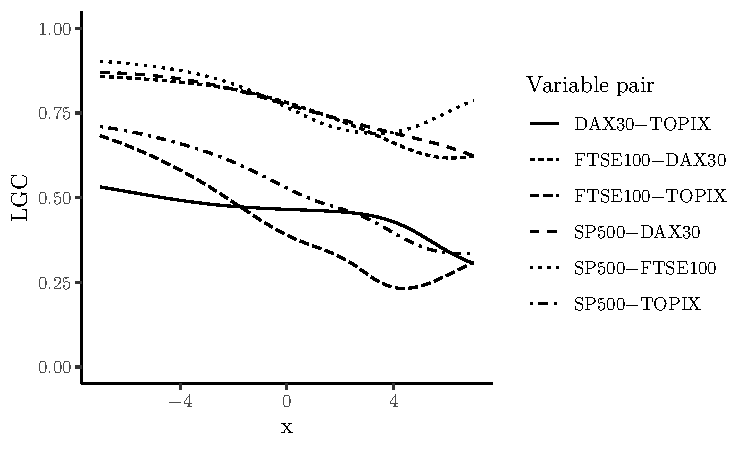
\includegraphics[width=\textwidth]{loccor-example}
      \caption{The estimated pairwise LGC for the stock \newline data along the diagonal.}
      \label{fig:lgc-plot1}
    \end{subfigure}
    \begin{subfigure}[t]{0.48\textwidth}
      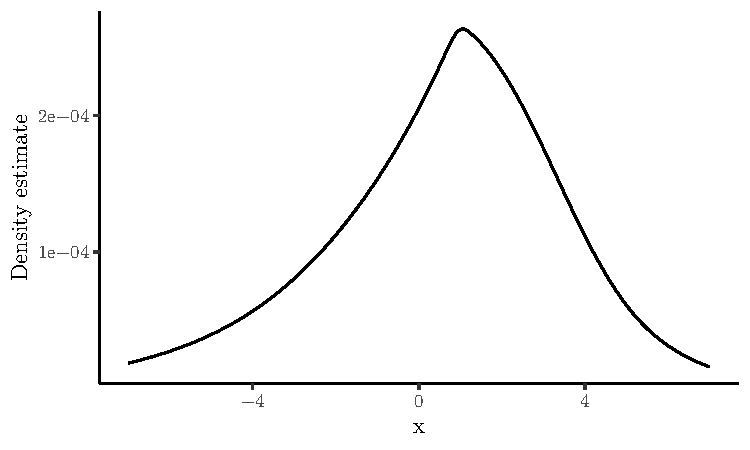
\includegraphics[width=\textwidth]{density-example}
      \caption{The corresponding joint density estimate of the four return series, plotted along the diagonal in $\mathbb{R}^4$.}
      \label{fig:lgc-plot2}
    \end{subfigure}
    \caption{Important output from the \code{dlg()-function}.}
    \label{fig:lgc-plot}
  \end{figure}

We start by introducing a basic function for estimating the LGC on a grid as described by \citet{otne:tjos:2017}, and thus also a probability density estimate. We create a grid, \code{x0}, having the same number of columns as the data in the code below. Note that we use the pipe operator \code{\%\textgreater{}\%} from the \CRANpkg{magrittr}-package \citep{bach:wick:2014} as well as functions from the \CRANpkg{dplyr}-package \citep{wick:fran:mull:2018} for easy manipulation of data frames. We then pass the grid and the lg-object containing our modelling choices to the \code{dlg()}-function in order to do the estimation.

\begin{example}
R> # Create an lg-object
R> lg_object <- lg_main(x = stock_data %>% select(-Date),
R+                      est_method = "1par",
R+                      bw_method = "plugin",
R+                      transform_to_marginal_normality = TRUE)
R> 
R> # Construct a grid diagonally through the data.
R> grid_size <- 100
R> x0 <- stock_data %>% 
R+   select(-Date) %>% 
R+   apply(2, function(y) seq(from = -7,
R+                            to = 7,
R+                            length.out = grid_size))
R> 
R> # Estimate the local Gaussian correlation on the grid
R> density_object <- dlg(lg_object, grid = x0)
\end{example}
The last line of code creates a list containing a number of elements. The two most important are \code{\$loc\_cor}, which is a matrix of local correlations having one row per grid point and one column per \emph{pair of variables} (the columns correspond to the rows in \code{density\_object\$pairs}), as well as \code{\$f\_est}, which is a vector containing the estimate \(\widehat f_X(x)\) of the joint density \(f_X(x)\) in the grid points specified in \code{x0}. The estimated local correlations for this example is plotted in Figure \ref{fig:lgc-plot1}, and the corresponding density estimate is plotted (along the diagonal \(x_1=x_2=x_3=x_4=x\)) in Figure \ref{fig:lgc-plot2}.

The list \code{density\_object} contains the estimated standard deviations of the local correlations in \code{\$loc\_cor\_sd}, as well
as lower and upper confidence bands \code{\$loc\_cor\_lower} and \code{\$loc\_cor\_upper} at the 95\% level. We refer to Table \ref{tab:dlg} for a complete overview of the arguments to \code{dlg()}.

Note that the configuration \code{transform\_to\_marginal\_normality\ =\ TRUE} and \code{est\_method\ =\ 5par} in the bivariate case coincides with the situation considered by \citet{tjos:huft:2013}. In that case, \code{dlg()} serves as a wrapper for the function \code{localgauss()} in the \CRANpkg{localgauss}-package \citep{bere:klep:tjos:2014}.

Obtaining the estimate of a conditional density using the \citet{otne:tjos:2018} algorithm described in Section \ref{chap:background} is very similar, but one must take particular care of the \emph{ordering} of the variables in the data set. The estimation function, \code{clg()}, will \emph{always} assume that the free variables come first, and that the conditioning variables come last. Let us illustrate this in the following code chunk by estimating the joint conditional density of S\&P500 and FTSE100, given that DAX30 = TOPIX = 0.

\renewcommand{\arraystretch}{1.2}
\begin{table}[t!]
\centering
\begin{tabular}{lll}
\toprule
Argument & Explanation & Default value \\
\midrule
\code{lg{\textunderscore}object} & The lg-object created by \code{lg{\textunderscore}main()} & \\
\code{grid} & The evaluation points for the LGC & \code{NULL} \\
\code{level} & Level for confidence bands & 0.95\\ 
\code{normalization} & The estimated density does not integrate to one by & \\ \code{{  \textunderscore}points} & construction. \code{dlg()} will generate the given number   & \\ & of normal variables, having  the same moments as   & \\ &  the data, approximate  $\int \widehat f_X(x)\,\textrm{d}x$ by a Monte Carlo  & \\ & integral, and then normalize the density estimate  & \\ & accordingly & \\ \code{NULL} \\
\code{bootstrap} & Calculate bootstrapped confidence intervals instead& \\ &  of asymptotic expressions & \code{FALSE} \\
\code{B} & Number of bootstrap replicates & \code{500} \\
\bottomrule
\end{tabular}
\caption{Arguments to the \code{dlg()}-function}
\label{tab:dlg}
\end{table}

\begin{example}
R> # We must make sure that the free variables come first
R> returns1 <- stock_data %>% select(SP500, FTSE100, DAX30, TOPIX)
R> 
R> # Create the lg-object
R> lg_object <- lg_main(returns1,
R+                      est_method = "1par",
R+                      bw_method = "plugin",
R+                      transform_to_marginal_normality = TRUE)
R> 
R> # Create a grid
R> x0 <- returns1 %>% 
R+   select(SP500, FTSE100) %>% 
R+   apply(2, function(y) seq(from = -7,
R+                            to = 7,
R+                            length.out = grid_size))
R> 
R> # Calculate the conditional density
R> cond_density <- clg(lg_object, grid = x0, cond = c(0, 0))
\end{example}

The key argument in the call to \code{clg()} above is \code{cond\ =\ c(0,\ 0)}. This means that the last two variables are conditioning variables (and hence that the first \(4-2=2\) variables are free), and that the value of the conditioning variables are fixed at DAX30 = 0 and TOPIX = 0 respectively. This also means that the number of columns in the grid \code{x0} plus the number of elements in \code{cond} must equal the number of variables \(p\) in the data set, and the call to \code{clg()} will result in an error message if this requirement is not fulfilled. Apart from \code{cond}, the \code{clg()}-function takes exactly the same arguments as \code{dlg()} listed in Table \ref{tab:dlg}, and the conditional density estimate in our example is available in the vector \code{cond\_density\$f\_est}.

\subsection{Tests for independence}
\label{chap:indtests}

Three independence tests based on the LGC have appeared in the literature thus far:

\begin{enumerate}
\def\labelenumi{\arabic{enumi}.}
\item
  A test for independence between the stochastic variables \(X_1\) and \(X_2\) based on iid data, cf. \citet{bere:tjos:2014}.
\item
  A test for serial independence between \(X_t\) and \(X_{t-k}\) within a time series \(\{X_t\}\), cf. \citet{laca:tjos:2017}. 
\item
  A test for serial cross-dependence between \(X_t\) and \(Y_{t-k}\) for two time series \(\{X_t\}\) and \(\{Y_t\}\), cf. \citet{laca:tjos:2018}.
\end{enumerate}
As we noted in Section \ref{chap:background}, their practical implementations are very similar, and the \CRANpkg{lg}-package provides the function \code{ind\_test()} to perform the tests. Let us first consider the iid case, and generate 500 observations \code{test\_x} from the well known parabola model \(X_2 = X_1^2 + \varepsilon\), where both \(X_1\) and \(\varepsilon\) are independent and standard normal. In this case, \(X_1\) and \(X_2\) are uncorrelated, but obviously strongly dependent. \citet{bere:tjos:2014} considers mainly the full bivariate fit to the raw data, which we easily encode into the lg-object as before. The implementation of the test using 100 bootstrap replicates is shown below.

\begin{example}
R> # Make the lg-object
R> lg_object <- lg_main(test_x, 
R+                      est_method = "5par",
R+                      transform_to_marginal_normality = TRUE)
R> # Perform the independence test
R> test_result <- ind_test(lg_object, n_rep = 100)
R> # Print out the p-value of the test
R> test_result$p_value

[1] 0
\end{example}
This may take a few minutes due to the bootstrapping. We can further specify the function \(h\) and the integration area \(S\) in the test
statistic \eqref{eq:test-statistic1}, see Table \ref{tab:indtest} for details.

\renewcommand{\arraystretch}{1.2}
\begin{table}[t!]
\centering
\begin{tabular}{lll}
\toprule
Argument & Explanation & Default value \\
\midrule
\code{lg{\textunderscore}object} & The lg-object created by \code{lg{\textunderscore}main()} & \\
\code{h} & The function $h(\cdot)$ in (\ref{eq:test-statistic1}) & \code{function(x) x{\textasciicircum}2} \\
\code{S} & The integration area $S$ in (\ref{eq:test-statistic1}). Must & \code{function(x)} \\ & be a logical function on potential  & \code{  as.logical(rep(1,} \\ & grid points in $\mathbb{R}^2$ & \code{    nrow(x)))} \\
\code{bootstrap} & The bootstrap method, must & \\ \code{  {\textunderscore}type} & be either \code{"plain"}, \code{"block"} or \code{"stationary"} & \code{"plain"} \\
\code{block} & Block length for the block bootstrap, &\\ \code{  {\textunderscore}length}& mean block length for the stationary &\\& bootstrap. Calculated by \code{np::b.star()} &\\& \citep{hayf:raci:2008} if not provided & \code{NULL} \\
\code{n{\textunderscore}rep} & Number of bootstrap replicates & 1000 \\
\bottomrule
\end{tabular}
\caption{Arguments to the \code{ind{\textunderscore}test()}-function}
\label{tab:indtest}
\end{table}


The only difference when testing for serial independence within a time series \(\{X_t\}\) is to create a two-column data set consisting of
\(X_t\) and \(X_{t-k}\). For example, if we wish to perform this test for \(k=1\) for one of the variables in the stock-exchange series,
create the matrix of observations as below, and proceed exactly as in the iid case.

\begin{example}
R> returns2 <- stock_data %>% select(SP500) %>% 
R+   mutate(sp500_lagged = lag(SP500))
\end{example}

Finally, the only thing that we must alter in order to perform the third test for serial cross-dependence is the bootstrap method. \citet{laca:tjos:2018} consider two options here, the block bootstrap with either fixed \citep{kuns:1989} or random \citep{poli:roma:1994} block sizes, and this choice is specified by choosing \code{bootstrap\_type\ =\ "block"} or \code{bootstrap\_type\ =\ "stationary"}, respectively, in the call to \code{ind\_test()}.

\subsection{Test for financial contagion}\label{chap:cont}

Assume that we observe two financial time series \(\{X_t\}\) and \(\{Y_t\}\) at times \(t = 1,\ldots,T\), and that some crisis occurs at time \(T^* < T\). As described in Section \ref{chap:background}, \citet{stov:tjos:huft:2014} measure the local correlation between \(\{X_t\}\) and \(\{Y_t\}\) \emph{before} and \emph{after} \(T^*\), and take significant differences between these measurements as evidence against the null hypothesis of no linkage, or contagion, between the time series. In order to implement this test using the \CRANpkg{lg}-package, one must create \emph{two} lg-objects: one for the observations covering the non crisis period and one covering the crisis period. We do not enter a discussion here how to empirically identify such time periods; this is a job that must be done by the practitioner before performing the statistical test.

Let us illustrate the implementation of this test by looking at the same financial returns data that we have used in preceding sections, but this time we will, in the spirit of \citet{stov:tjos:huft:2014}, concentrate on \emph{GARCH(1,1)-filtrated daily returns on the S\&P500 and FTSE100 indices from 2 January 1985 to 29 April 1987} in order to test for financial contagion between the US and UK stock markets following the global stock market crash of 19 October 1987 (``Black Monday''). Assume that these observations are loaded into the R workspace as the \(n_1 \times 2\) data frame \code{x\_nc} containing the observations covering the \(n_1 = 728\) days preceding the crisis , and the \(n_2 \times 2\) data frame \code{x\_c} containing the observations covering the \(n_2 = 140\) consecutive trading days starting on \emph{Black Monday} (see the online code supplement for details concerning the GARCH-filtration and data processing). In the code below we construct one lg-object for each of these data frames with configuration matching the setup used by \citet{stov:tjos:huft:2014}, and perform the test by means of the \code{cont\_test()}-function.

This function returns a list containing the estimated \(p\)-value as well as other useful statistics, including the empirical local correlations measured in the two time periods. See Table \ref{tab:arguments-cont-test} for details concerning other arguments that may be passed to this function.

\renewcommand{\arraystretch}{1.2}
\begin{table}[t!]
\centering
\begin{tabular}{lll}
\toprule
Argument & Explanation & Default value \\
\midrule
\code{lg{\textunderscore}object{\textunderscore}nc} & The lg-object covering the non-crisis period & \\
\code{lg{\textunderscore}object{\textunderscore}c} & The lg-object covering the crisis period & \\
\code{grid{\textunderscore}range} & Range of diagonal for measuring the LGC & (5\%, 95\%) quantiles \\
\code{grid{\textunderscore}length} & The number of grid points to use & 30 \\
\code{n{\textunderscore}rep} & Number of bootstrap replicates & 1000 \\
\code{weight} & Weight function & \code{function(y)} \\ 
&& \code{  rep(1, nrow(y))} \\
\bottomrule
\end{tabular}
\caption{Arguments to the \code{cont{\textunderscore}test()-function}}
\label{tab:arguments-cont-test}
\end{table}

\begin{example}
R> # Create the two lg-objects
R> lg_object_nc <- lg_main(x_nc, 
R+                         est_method = "5par",
R+                         transform_to_marginal_normality = FALSE)
R> 
R> lg_object_c <- lg_main(x_c, 
R+                         est_method = "5par",
R+                         transform_to_marginal_normality = FALSE)
R> 
R> # Run the test with a limited number of bootstrap replicates for 
R> # demonstration purposes.
R> result <- cont_test(lg_object_nc, lg_object_c, n_rep = 20)
R> 
R> # Print out the p-value
R> result$p_value

[1] 0
\end{example}

\subsection{Partial local correlation}
\label{chap:partial}

Consider finally the work by \citet{otne:tjos:2019} who take the off-diagonal element in the local correlation matrix corresponding to the local conditional covariance matrix \eqref{eq:cond-sig} or \eqref{eq:cond-sig-trans} as a local measure of conditional dependence between two stochastic variables \(X^{(1)}\) and \(X^{(2)}\) given the stochastic vector \(X^{(3)}\), and furthermore, in the case with data having been transformed to marginal standard normality, take the statistic
\[T^{CI}_{n, b} = \int h(\widehat\alpha(z)) \, \textrm{d}F_n(z)\]
as a measure of \emph{global} conditional dependence. To this end, the \CRANpkg{lg}-package provides two functions. The first, \code{partial\_cor()}, calculates the local partial correlations as well as their estimated standard deviations, on a specified grid in the \((x^{(1)}, x^{(2)}, x^{(3)})\)-space, and is essentially a wrapper function for the \code{clg()}-function presented in Section \ref{chap:density}. See Table \ref{tab:arguments-partial-cor} for details. The second function, \code{ci\_test()}, performs a test for conditional independence between the first two variables in a data set given the remaining variables.

\renewcommand{\arraystretch}{1.2}
\begin{table}[p]
\centering
\begin{tabular}{lll}
\toprule
Argument & Explanation & Default value \\
\midrule
\texttt{lg{\textunderscore}object} & The lg-object created by \texttt{lg{\textunderscore}main()}  & \\
\texttt{grid} & The evaluation points for the LGPC, \textbf{must} be a & \\
& \qquad  data frame or matrix having 2 columns  & \texttt{NULL} \\
\texttt{cond} & Vector with fixed values for $X^{(3)}$ & \texttt{NULL} \\
\texttt{level} & Significance level for approximated confidence bands & 0.95 \\
\bottomrule
\end{tabular}
\caption{Arguments to the \texttt{partial{\textunderscore}cor()-function}}
\label{tab:arguments-partial-cor}
\end{table}

\begin{table}[p]
\centering
\begin{tabular}{lll}
\toprule
Argument & Explanation & Default value \\
\midrule
\texttt{lg{\textunderscore}object} & The lg-object created by \texttt{lg{\textunderscore}main()}  & \\
\texttt{h} & The function $h(\cdot)$ in (\ref{eq:ci-test-statistic}) & \texttt{function(x) x{\textasciicircum}2} \\
\texttt{n{\textunderscore}rep} & Number of bootstrap replicates & 500 \\
\bottomrule
\end{tabular}
\caption{Arguments to the \texttt{ci{\textunderscore}test()-function}}
\label{tab:arguments-ci-test}
\end{table}

It is well known in the econometrics literature that conditional independence tests are instrumental in the empirical detection of Granger causality \citep{gran:1980}. For example, if we continue to concentrate on the monthly stock returns data that we have already loaded into memory, we may test whether 
\begin{equation} 
\textrm{H}_0: \qquad R_{\textrm{FTSE100}, t} \perp R_{\textrm{SP500}, t-1} \,\, | \,\, R_{\textrm{FTSE100}, t-1}
\label{eq:cond-ind-test}
\end{equation} 
in the period starting in January 2009, the converse of which is a sufficient, but not necessary, condition for \(R_{\textrm{SP500}, t}\) Granger causing \(R_{\textrm{FTSE100}, t}\). We perform the test by running the code below, where \code{x} is a data frame having the following columns strictly ordered as \(R_{\textrm{FTSE100}, t}\), \(R_{\textrm{SP500}, t-1}\) and \(R_{\textrm{FTSE100}, t-1}\) (see the online supplement for the pre-processing of data). 

The critical values of this test are calculated using the bootstrap under the null hypothesis by independently resampling replicates from
the conditional density estimates \(\widehat f_{X^{(1)|X^{(3)}}}(x^{(1)}|x^{(3)})\) and \(\widehat f_{X^{(2)|X^{(3)}}}(x^{(2)}|x^{(3)})\), as obtained by the \code{clg()}-function, using an approximated accept-reject algorithm. In order to avoid excessive optimization of the local likelihood function \eqref{eq:loclik}, we estimate \(f_{X^{(1)|X^{(3)}}}\) and \(f_{X^{(2)|X^{(3)}}}\) on the univariate regular grids \(x_0^{(1)}\) and \(x_0^{(2)}\) respectively (while keeping \(x^{(3)}\) fixed at the observed values of \(X^{(3)}\)), and produce interpolating functions \(\tilde f_{X^{(1)|X^{(3)}}}\) and \(\tilde f_{X^{(2)|X^{(3)}}}\) using cubic splines. It is much less computationally intensive to generate replicates from \(\tilde f\) than directly from \(\widehat f\).

We refer to the documentation of the \CRANpkg{lg}-package for details on how to finely tune the behavior of the bootstrapping algorithm by altering the arguments of the \code{ci\_test()}-function, and rather describe the arguments most suitable for modifications by the user in Table \ref{tab:arguments-ci-test}.

\begin{example}
R> # Create the lg-object
R> lg_object <- lg_main(returns4)
R> 
R> # Perform the test
R> test_result <- ci_test(lg_object, n_rep = 100)
R> 
R> # Print out result
R> test_result$p_value

[1] 0.71
\end{example}
The conditional independence test does not provide evidence against the null hypothesis \eqref{eq:cond-ind-test}.

\section{Graphics}\label{chap:graphics}

We conclude this article by describing the \code{corplot()} function, that may be used to draw dependence maps such as those displayed in Figure \ref{fig:initial-example}. \citet{bere:klep:tjos:2014} report on such capabilities in the \CRANpkg{localgauss}-package, but the possibility of creating dependence maps was unfortunately removed from \CRANpkg{localgauss} in the latest version 0.4.0 due to incompatibilities with the \CRANpkg{ggplot2} \citep{wick:2016} plotting engine. We make up for this loss by providing \code{corplot()}, a function that plots the estimated local correlations as provided by \code{dlg()}, or the estimated local \emph{partial} correlations as provided by \code{partial\_cor()}.

The plotting function is highly customizable and provides a number of options covering most basic graphical options. Users well versed in the \CRANpkg{ggplot2}-package may also modify the graphical object returned by corplot in the standard way by adding layers as demonstrate in the example below.

In the first example we generate a set of bivariate normally distributed data using the \CRANpkg{mvtnorm}-package \citep{gentz:etal:2018} and estimate the local Gaussian correlation on a regular \code{grid} using the \code{dlg()}-function. Passing the resulting \code{dlg\_object} to \code{corplot()} without further arguments results in Figure \ref{fig:graphics1}.

\begin{example}
R> # Make a regular grid in the domain of the distribution
R> grid <- expand.grid(seq(-3, 3, length.out = 7),
R+                     seq(-3, 3, length.out = 7))
R> 
R> x <- mvtnorm::rmvnorm(500, sigma = matrix(c(1, rho, rho, 1), 2))
R> lg_object <- lg_main(x, 
R+                      est_method = "5par", 
R+                      transform_to_marginal_normality = FALSE,
R+                      plugin_constant_joint = 4)
R> dlg_object <- dlg(lg_object, grid = grid)
R> 
R> # Make a dependence map using default setup
R> corplot(dlg_object1)
\end{example}


We may tweak the appearance of our dependence map by passing further arguments to \code{corplot()}. Some of the options are demonstrated in the code chunk below, in which we, for example, superimpose the observations (by setting \code{plot\_obs\ =\ TRUE)} as well as preventing the the estimated local correlations from being plotted in areas without data. The latter option is available through the argument \code{plot\_thres}, which works by calculating a bivariate kernel density estimate \(\tilde f(x_1, x_2)\) for the pair of  variables in question, and only allowing \(\widehat \rho(x_1,x_2)\) to be plotted if \(\tilde f(x_1,x_2)/\max\tilde f(\cdot) >\) \code{plot\_thres}. Adding layers to a dependence map using the ordinary \CRANpkg{ggplot2} syntax works as well, which we demonstrate in Figure \ref{fig:graphics2} by changing the \CRANpkg{ggplot2} theme.

The plotting function works in the same way when plotting the local partial correlations returned by \code{partial\_cor()}, and the arguments of \code{corplot()} are summarized in Table \ref{tab:arguments-corplot}.

\renewcommand{\arraystretch}{1.2}
\begin{table}[p]
\centering
\begin{tabular}{lll}
\toprule
Argument & Explanation & Default value \\
\midrule
\code{dlg{\textunderscore}object} & The object created by \code{dlg()} or \code{partial{\textunderscore}cor()}  & \\
\code{pair} & Which pair to plot if more than two variables & 1 \\
\code{gaussian{\textunderscore}scale} & Logical. Plot on the marginal st. normal scale? & \code{FALSE} \\
\code{plot{\textunderscore}colormap} & Logical. Plot the colormap? & \code{TRUE} \\
\code{plot{\textunderscore}obs} & Logical. Superimpose observations? & \code{FALSE} \\
\code{plot{\textunderscore}labels} & Logical. Plot labels on dependence map? & \code{TRUE} \\
\code{plot{\textunderscore}legend} & Logical. Add legend? & \code{FALSE} \\
\code{plot{\textunderscore}thres} & Threshold for plotting the estimated LGC & 0 \\
\code{alpha{\textunderscore}tile} & Transparency of color tiles & 0.8 \\
\code{alpha{\textunderscore}point} & Transparency of points & 0.8 \\
\code{low{\textunderscore}color} & Color representing $\widehat\rho = -1$ & \code{"blue"}\\
\code{high{\textunderscore}color} & Color representing $\widehat\rho = +1$ & \code{"red"}\\
\code{break{\textunderscore}int} & Break interval for color coding & 0.2 \\
\code{label{\textunderscore}size} & Size of labels in plot & 3 \\
\code{font{\textunderscore}family} & Font family for labels & \code{"sans"} \\
\code{point{\textunderscore}size} & Size of points, if plotted & \code{NULL} \\
\code{xlim}, \code{ylim} & Axis limits & \code{NULL} \\
\code{xlab}, \code{ylab} & Axis labels & \code{NULL} \\
\code{rholab} & Title of legend & \code{NULL} \\
\code{main}, \code{subtitle} & Title and subtitle of plot & \code{NULL} \\
\bottomrule
\end{tabular}
\caption{Arguments to the \code{corplot()}-function}
\label{tab:arguments-corplot}
\end{table}

\begin{example}
R> corplot(dlg_object1, 
R+         plot_obs = TRUE, 
R+         plot_thres = 0.01,
R+         plot_labels = FALSE,
R+         alpha_point = 0.3,
R+         main = "",
R+         xlab = "",
R+         ylab = "") +
R+   theme_classic()
\end{example}

\begin{figure}[p]
\centering 
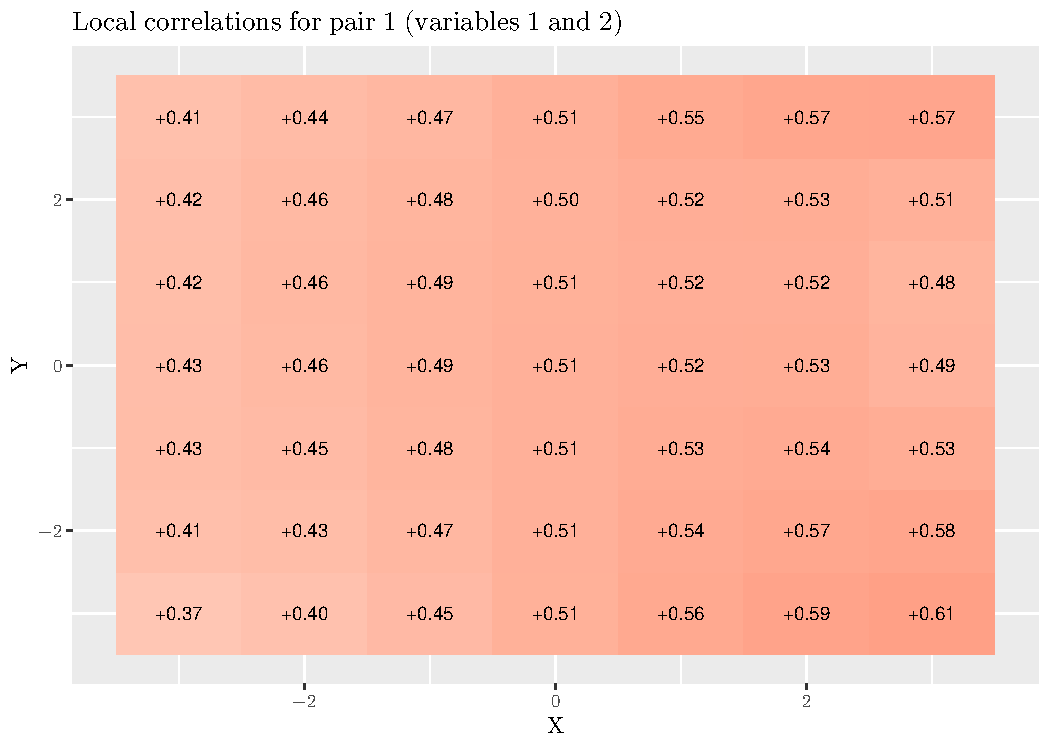
\includegraphics[width = \textwidth]{graphics1} 
\caption{Dependence map produced by \code{corplot()} using the default configuration}
\label{fig:graphics1}
\end{figure}


\begin{figure}[p]
\centering 
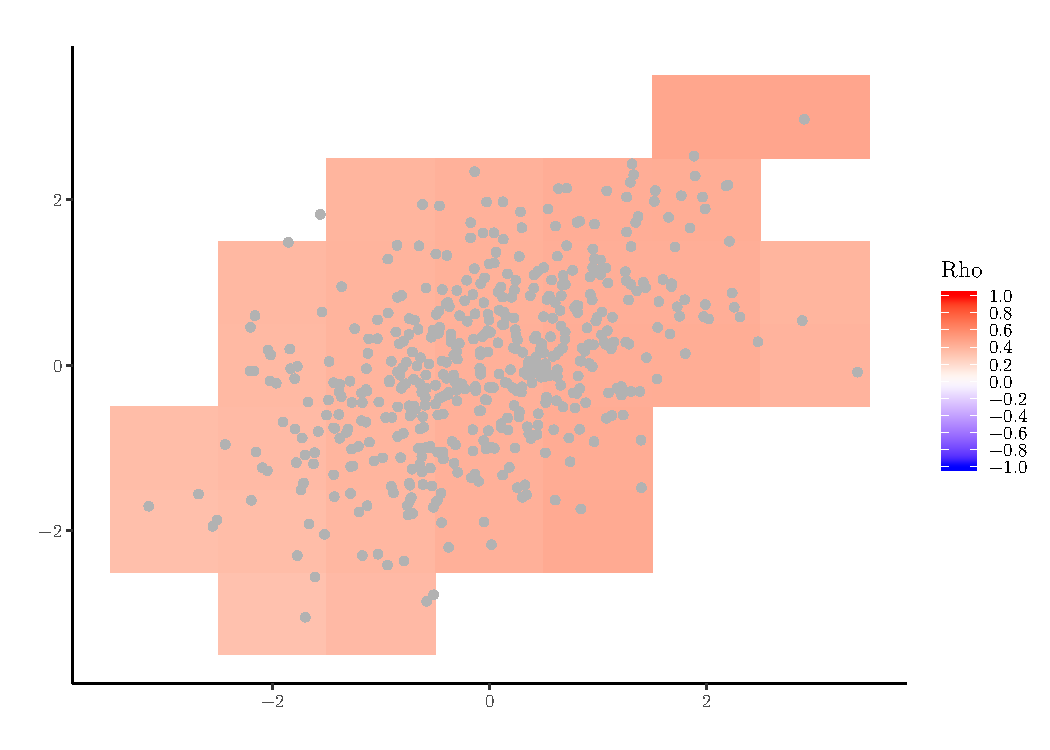
\includegraphics[width = \textwidth]{graphics2} 
\caption{Dependence map produced by tweaking the arguments of \code{corplot()}}
\label{fig:graphics2}
\end{figure}

\section{Conclusion} 

The statistical literature has seen a number of applications of local Gaussian approximations in the last decade, covering several topics in dependence modeling and inference, as well as the estimation of multivariate density and conditional density functions. In this paper, we demonstrate the implementation of these methods i the R programming language using the \CRANpkg{lg}-package, as well as the graphical representation of the estimated local Gaussian correlation. The package is complete, in the sense that all major methods that have been published within this framework is now easily accessible to the practitioner. The package is also modular; Future methodological developments using local Gaussian approximations may be added to the package with little effort. 

\bibliography{otneim}

\address{H{\aa}kon Otneim\\
  Department of Business and Management Science, \\
  NHH Norwegian School of Economics, \\
  Helleveien 30, 5045 BERGEN\\
  Norway\\
  \email{hakon.otneim@nhh.no}}

